\documentclass[notitlepage]{report}
\usepackage{geometry} % see geometry.pdf on how to lay out the page. There's lots.
\usepackage{natbib}
\usepackage{graphicx}
\usepackage{pdfpages}
\usepackage{url}
\geometry{a4paper} % or letter or a5paper or ... etc
% \geometry{landscape} % rotated page geometry

\makeatletter
\newcommand*{\toccontents}{\@starttoc{toc}}
\makeatother

% See the ``Article customise'' template for come common customisations

\begin{document}

\title{Supplementary Information 4 for \\ \emph{Cultural influences on word meanings revealed throughlarge-scale semantic alignment:}\\Cross-cultural analyses}
\author{Bill Thompson, Se\'{a}n Roberts \& Gary Lupyan}
\date{}
\maketitle

This document contains the supporting information on cross-cultural analyses for \emph{Cultural influences on word meanings revealed throughlarge-scale semantic alignment}.  Most of the contents are compiled R markdown documents, showing the R code for analysing the data. The full repository can be found here:\\
\url{https://github.com/seannyD/ImputeEACulturalDifferences}\\
The contents are as follows.  \\\\
\toccontents

\setcounter{chapter}{4}

\newpage
\section{Main cross-cultural analysis (Wikipedia data)}

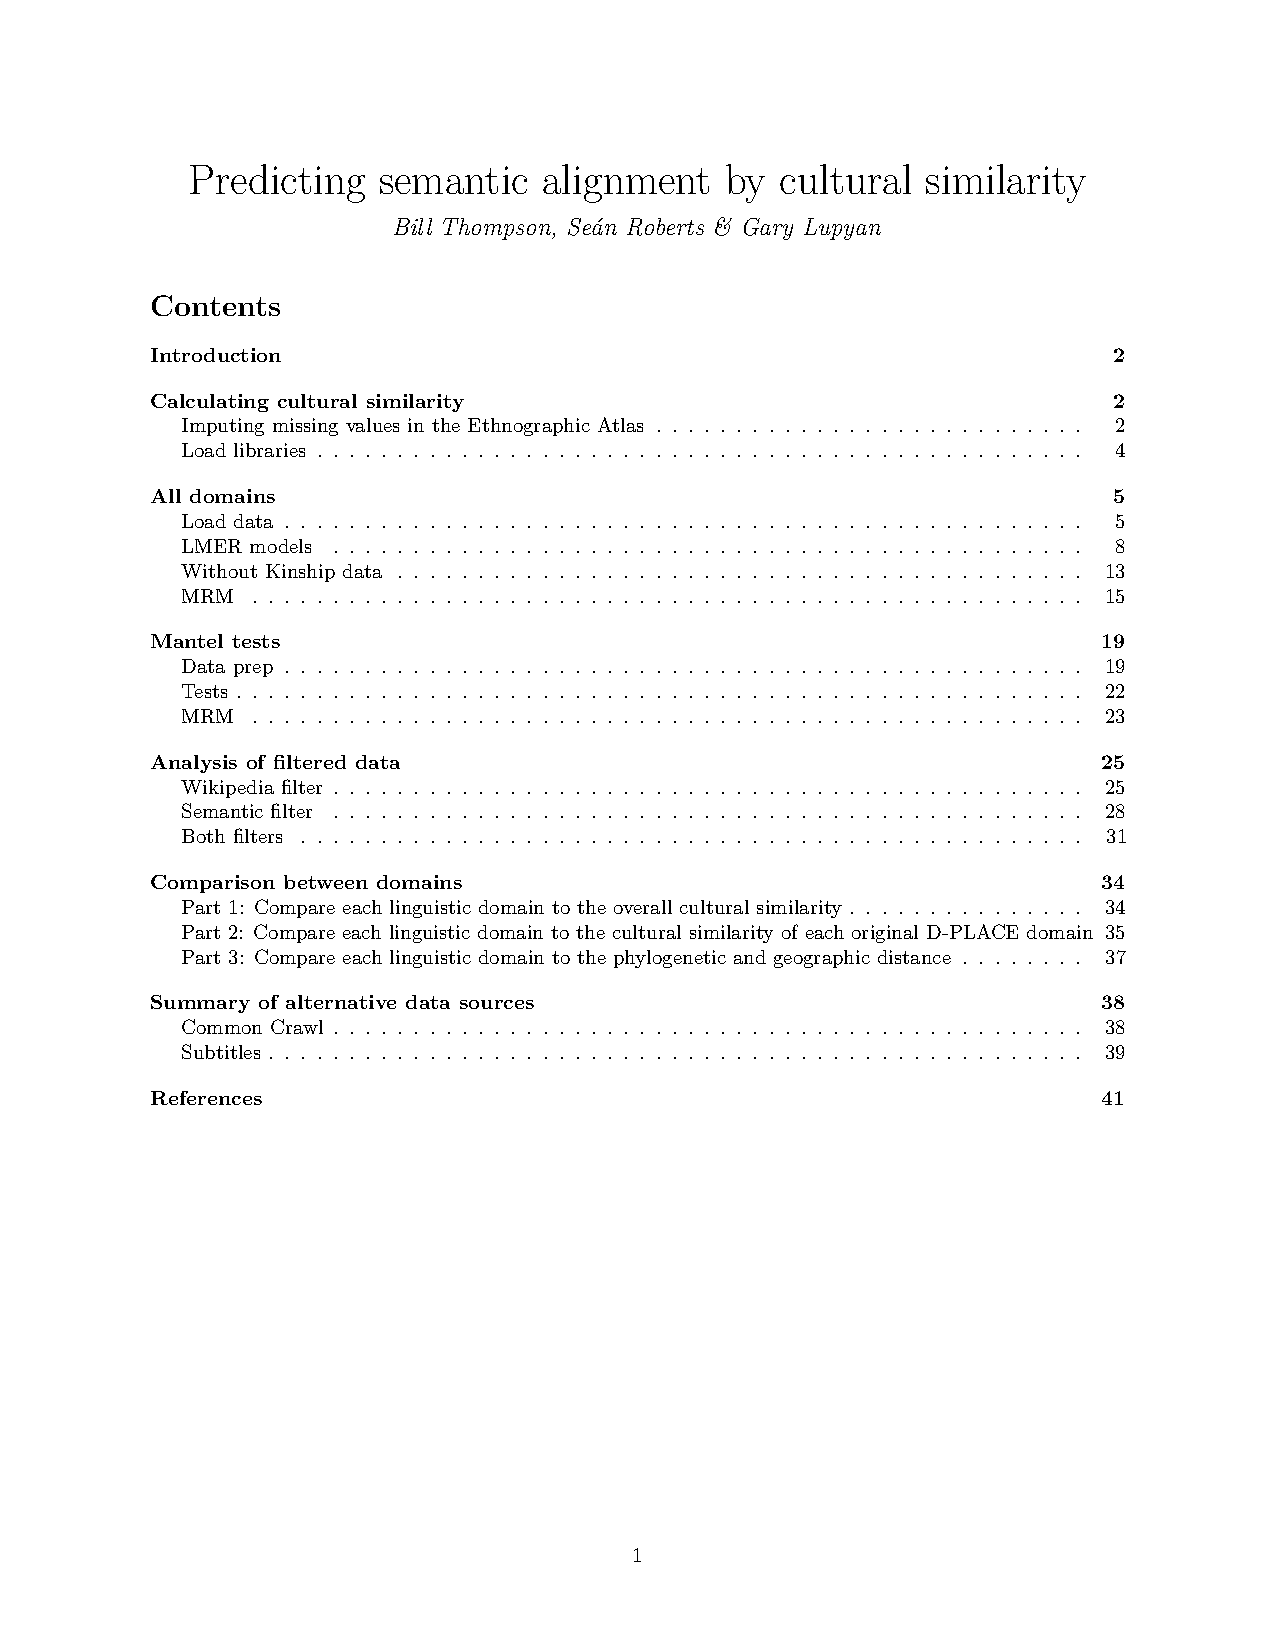
\includepdf[pages=-]{../analysis/MainAnalysis_analyseCorrelation_wikipedia.pdf}

\newpage
\section{Analysis of numerals}

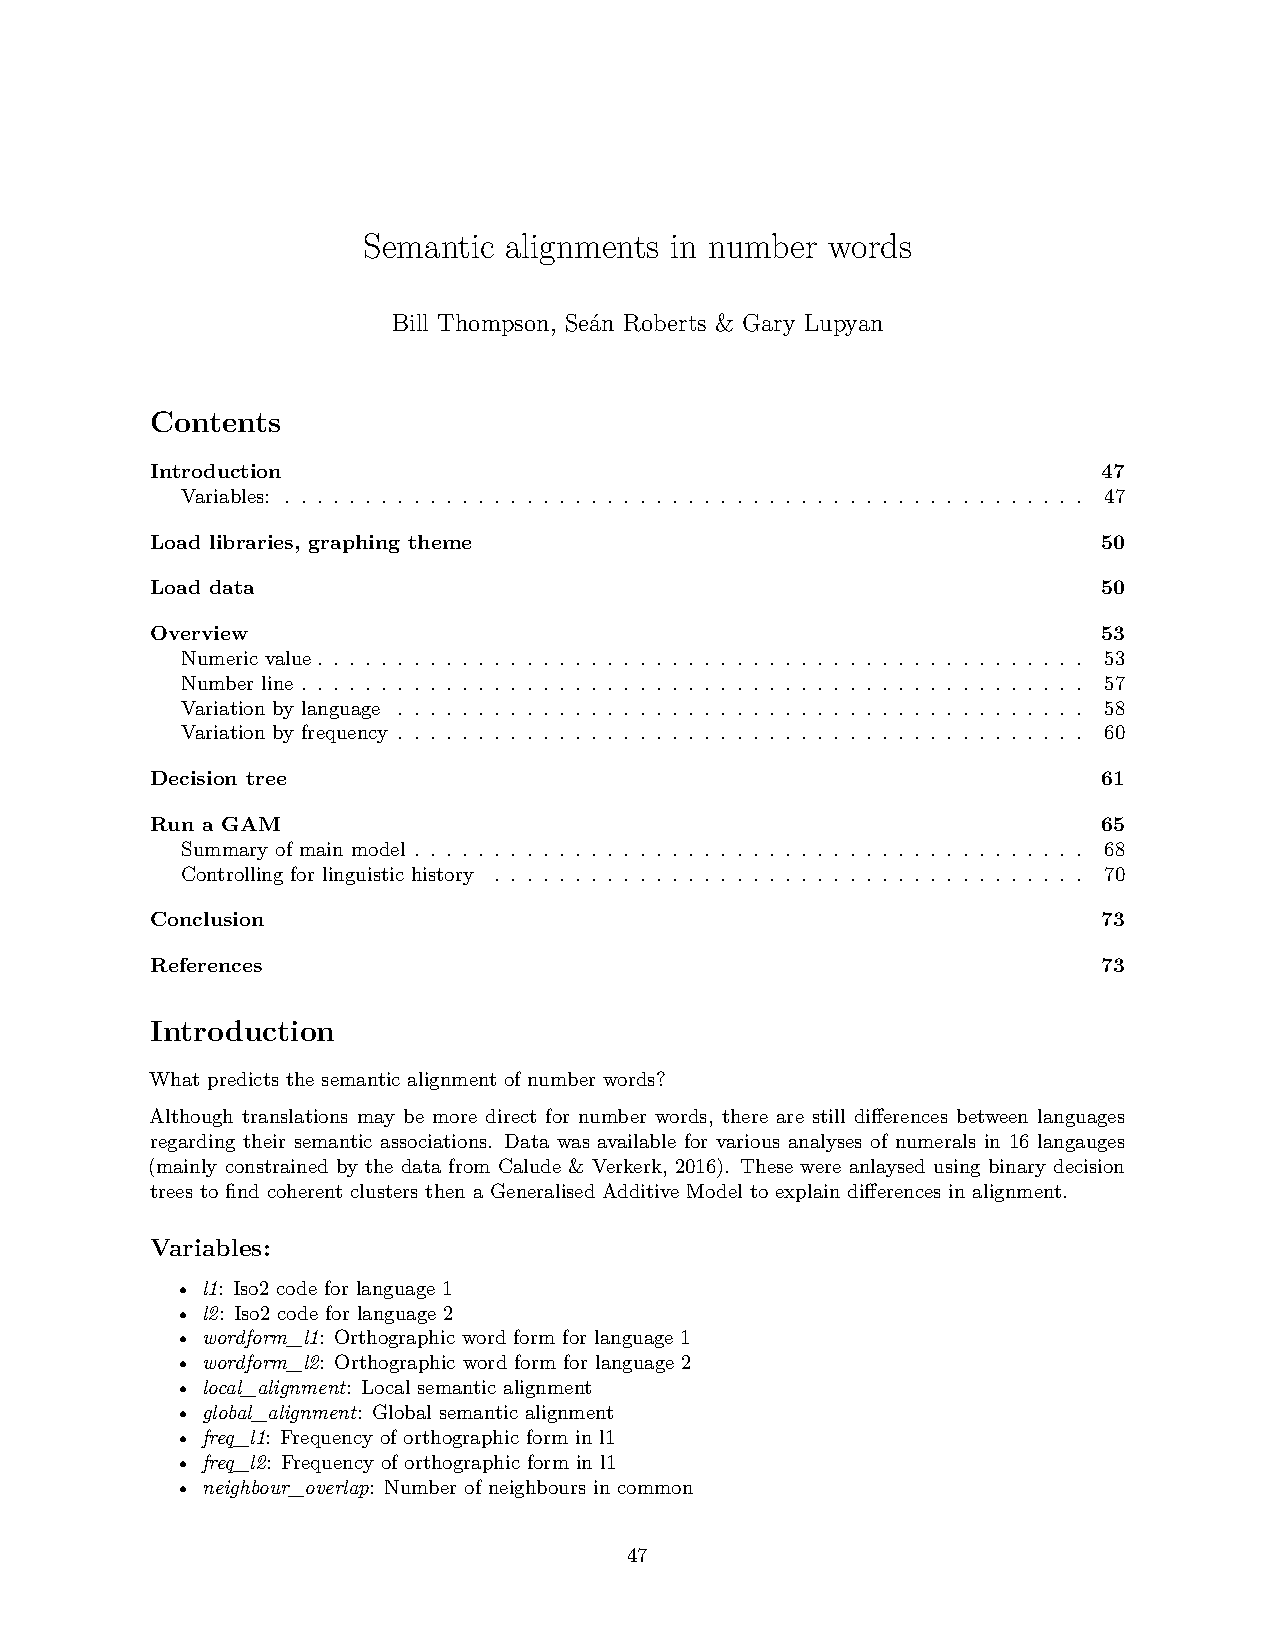
\includepdf[pages=-]{../analysis/numbers/number_alignment.pdf}

\clearpage
\newpage
\section{Neighbour net visualisation of semantic alignment}

The semantic alignment between languages was converted into a semantic distance and was visualised as a Neighbour Net using Splitstree (Huson \& Bryant, 2006). This was done on the data with both the language filter and the concept filter. The code for building the Neighbour Net and the resulting nexus file are here: \\ {\scriptsize \url{https://github.com/seannyD/ImputeEACulturalDifferences/blob/master/processing/makeSplitstreeNexusFile.R}}. \\ {\scriptsize \url{https://github.com/seannyD/ImputeEACulturalDifferences/blob/master/results/splitstree/LinguisticDistances.nex}}.

Neighbour Nets visualise a matrix of distances between individuals (in this case, individuals are languages). They attempt to draw a line between each pair of individuals whose length reflects the distances in the matrix.  A set of individuals that were all equally distant from each other would be represented as several lines of equal length originating from a single point, with the individuals placed at the tips (a `star' phylogeny).  If distances follow a strictly diverging, binary branching tree (pure vertical transmission), then the visualisation would look like a branching tree (a phylogeny), with more closely related individuals `clustered' together. However, many cases of cultural evolution also involve horizontal transmission, where there is transmission between individuals who have previously diverged. This leads to conflicting signals: individuals with elements inherited not just from their immediate ancestors, but from other parts of the tree. In a neighbour net, extra parallel lines are drawn along the underlying phylogeny structure. Ideally, the distance between two individuals will still be represented accurately by the shortest route between them following the lines. An individual with close ties to two other individuals will have alternative routes to reach each one. At the same time, a part of the tree that had only vertical transmission could be drawn as a phylogeny. This leads to a web-like structure that has properties of networks where there is horizontal signal but also some clustering properties of trees where there is vertical signal. For more on the use of neighbour nets in linguistics, see e.g. McMahon et al. (2007) or Skirgard et al., (2017). 

Figure \ref{fig:NNAll} shows the semantic distances for all languages in the sample (Delta score = 0.3844, Q-residual score = 0.0008379). Languages which are joined by short lines have higher semantic alignment (translation equivalents are closer in meaning).  Languages are roughly grouped by language family, with the Indo-European group being most clear, but also Uralic, Turkic and Afro-Asiatic groups visible. The figure also reflects geographic distances, with Persian and Armenian showing up on the ``Eastern'' side.  There is some clear conflicting signal for English between the Romance and Germanic, which reflects its mixed history (see e.g. McWhorter, 2008). This figure with languages from many different language families is somewhat misleading, since many languages that have high distances appear ``together'' in space (e.g. Basque and Korean), when in reality the distances along the lines are much further than for e.g. most Indo-European languages. Therefore, we also produced a Neighbour Net just for Indo-European languages.


Figure \ref{fig:NNIE} shows the semantic distances for Indo-European languages visualised as a neighbour-net (Delta score = 0.3062, Q-residual score = 0.003523). The semantic distances reflect established historical relationships, as shown by the labelling of the major sub-branches according to Glottolog (Hammarstrom et al.). Again, English shows conflicting signal between Germanic and Romance. There is a clear historical signal in the Slavic languages. Also, a split between `eastern' and `western' languages, with Romanian and Greek being halfway between the two.  Hindi, Armenian, Lithuanian and Greek are more removed from the rest historically, and that's reflected in the fact that they're placed `together', though actually the distance from Hindi to Armenian is much larger than for Russian to Ukrainian.

Some more speculative comments can also be made. The relationship between many languages reflects geographic proximity, such as the cline from Norwegian, Danish, German and Dutch. The proximity of Spanish and Catalan may also reflect contact and bilingualism. Romanian is an outlier in the romance languages and has a large amount of borrowed words from slavic languages (Schulte, 2009), so it's not suprising that it shows up on the edge of the Romance cluster. The proximity of Bulgarian and Greek may reflect geographical proximity and historical ties such as the Ottoman empire. The proximity of Armenian and Hindi is not predicted by linguistic family trees (e.g. Glottolog), but there is actually a history of contact, with trade leading to a historical Armenian population in Hindi-speaking places like Agra (e.g. Ferrier, 1973), and maybe more indirect borrowings through related languages (Pisowicz, 1995). 

\noindent
\textbf{References}

Huson, D.H. and Bryant, D. (2006) Application of Phylogenetic Networks in Evolutionary Studies, Mol. Biol. Evol., 23(2):254-267.

McWhorter, J. H. (2008) Our magnificent bastard tongue: The untold history of English. Penguin.

Hammarstr�m, H, Forkel, R, \& Haspelmath, M. (2019) Glottolog 4.0. Jena: Max Planck Institute for the Science of Human History.

McMahon, A., Heggarty, P., McMahon, R., \& Maguire, W. (2007). The sound patterns of Englishes: representing phonetic similarity. English Language \& Linguistics, 11(1), 113-142. 

Schulte, K. (2009) Loanwords in Romanian. In M. Haspelmath \& U. Tadmor, \emph{Loanwords in the World's Languages: A Comparative Handbook}. Walter de Gruyter. p. 243.

Skirg�rd, H., Roberts, S. G., \& Yencken, L. (2017). Why are some languages confused for others? Investigating data from the Great Language Game. PloS one, 12(4), e0165934.

Ferrier, R. W. (1973). The Armenians and the East India Company in Persia in the seventeenth and early eighteenth centuries. The Economic History Review, 26(1), 38-62.

Pisowicz, A. (1995). How did New Persian and Arabic Words Penetrate the Midle Armenian Vocabulary? Remarks on the Material in Kostandin Erznkac ?i?s Poetry?. New Approaches to Medieval Armenian Language and Literature, 3, 95.

\makeatletter 
\renewcommand{\thefigure}{4.3.\@arabic\c@figure}
\makeatother

\begin{figure}[hb]
\begin{center}
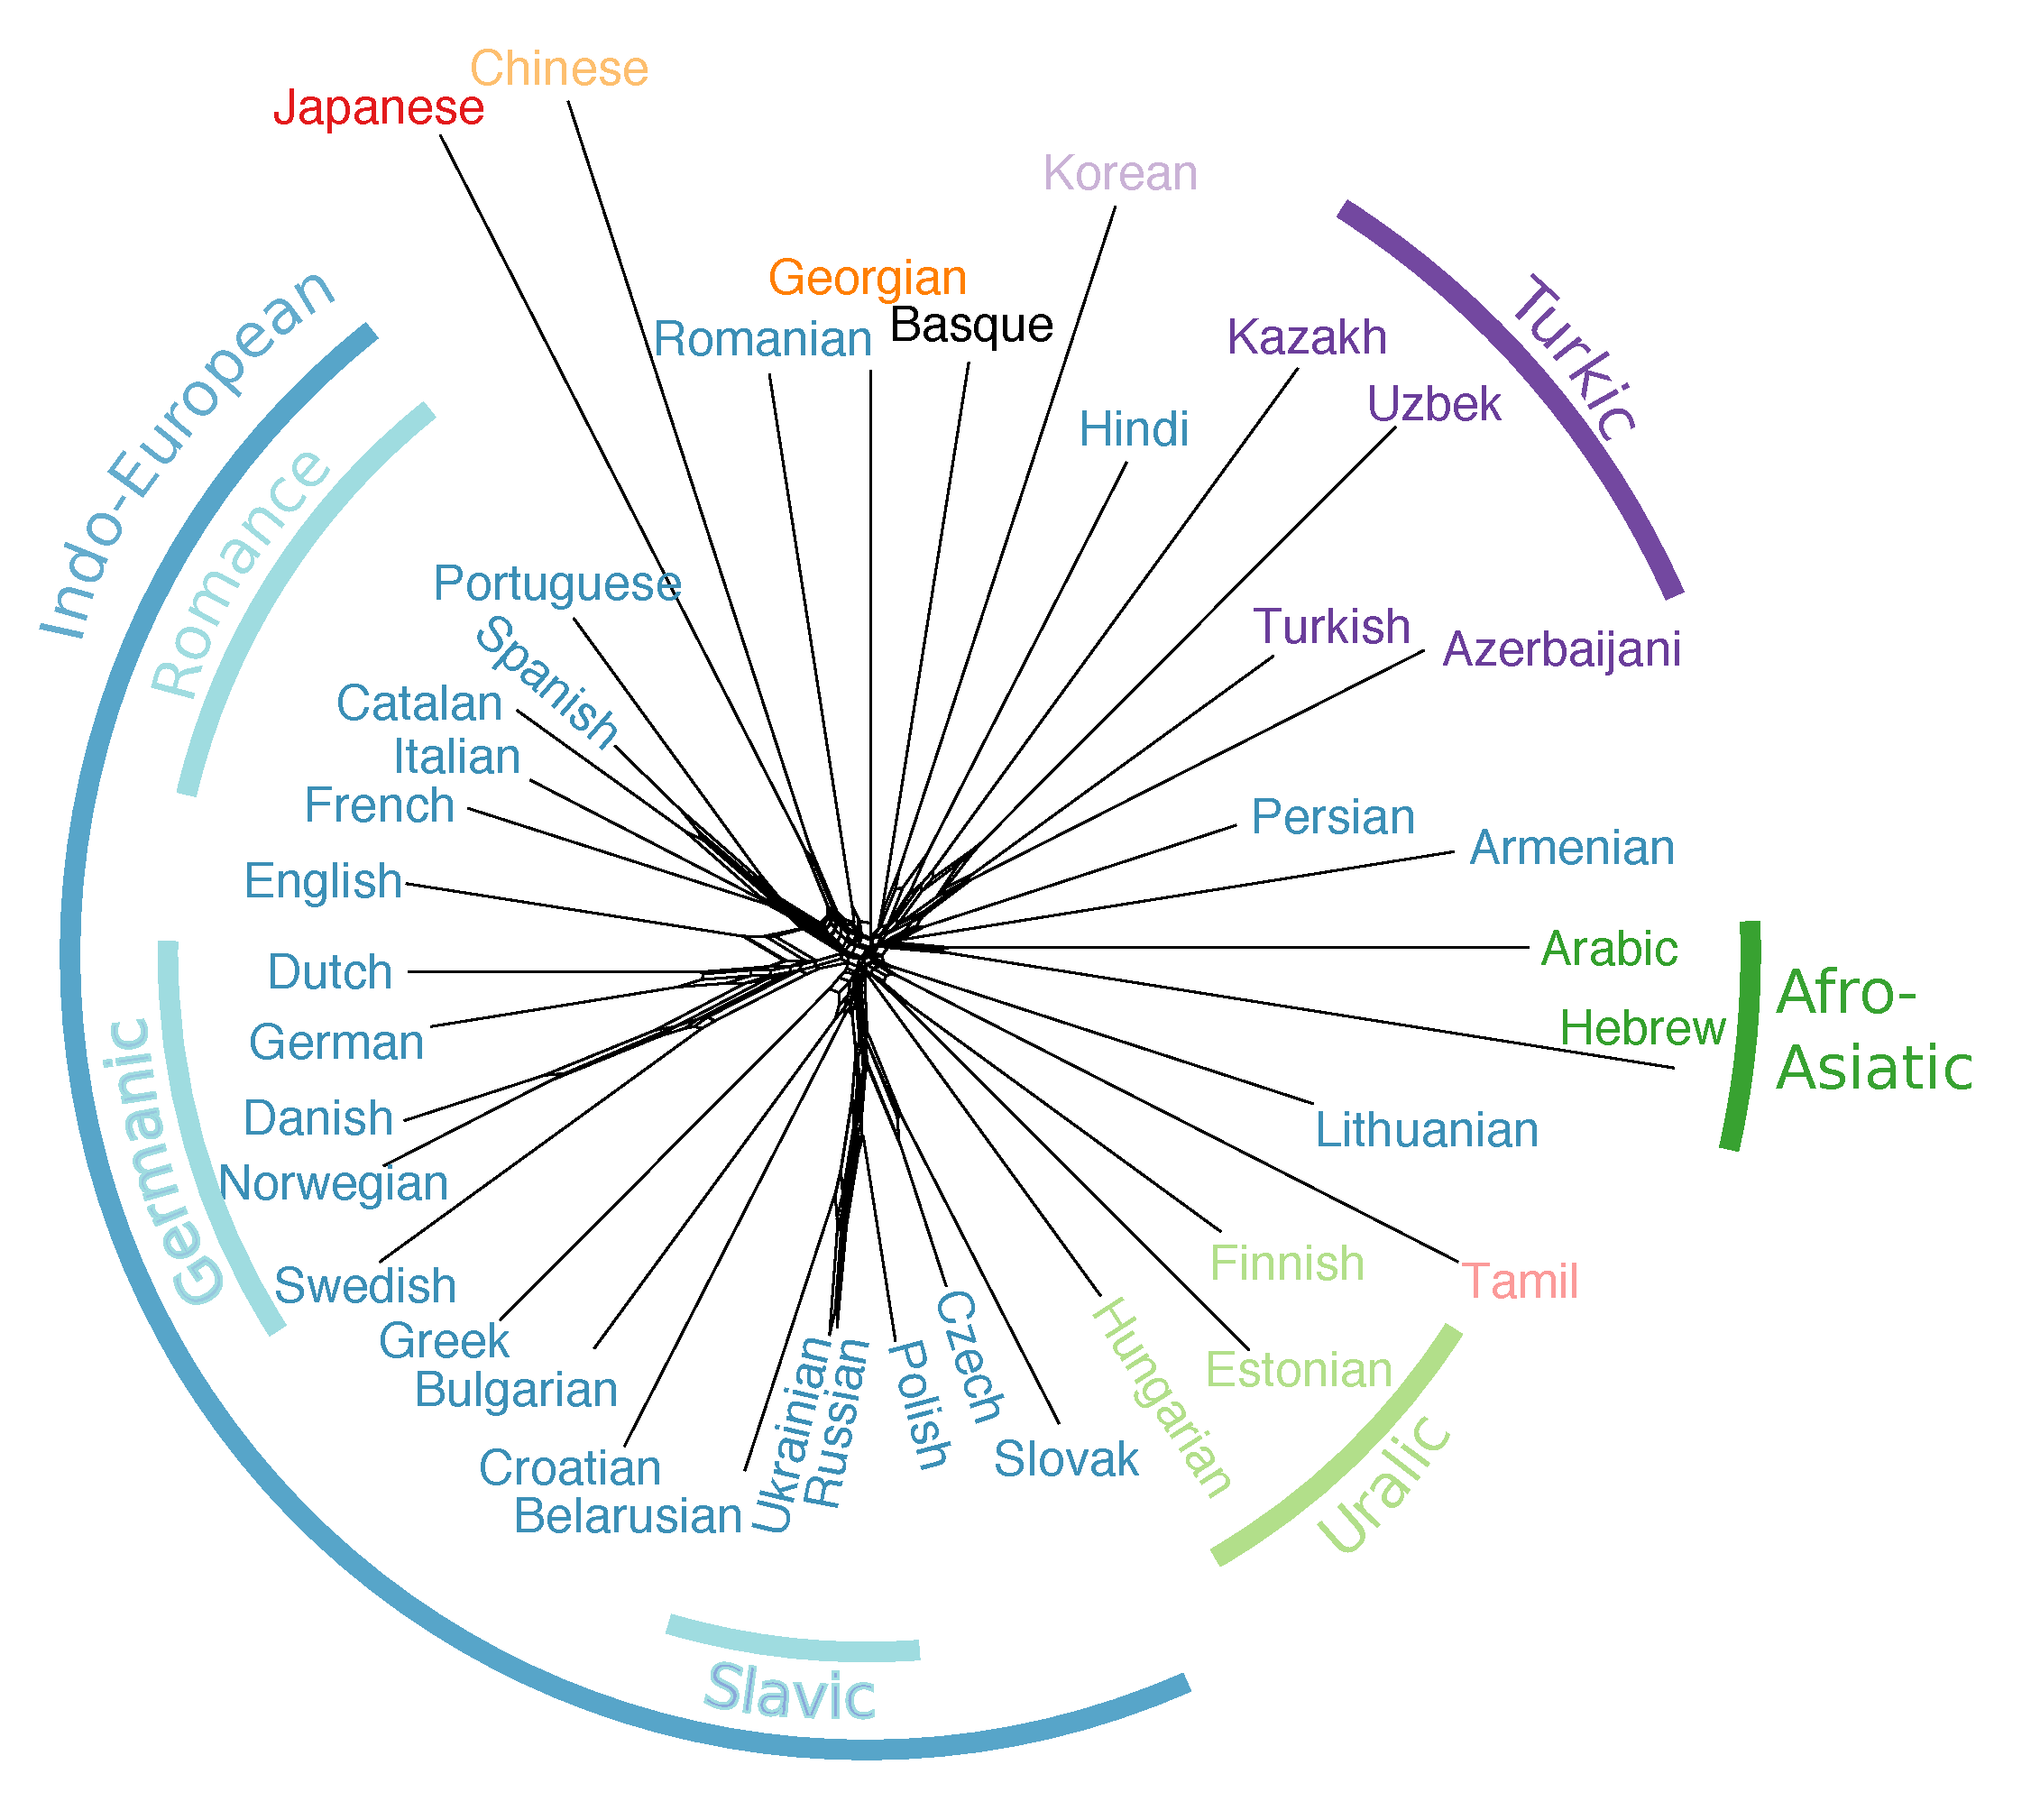
\includegraphics[width=\linewidth]{../results/splitstree/LinguisticDistances2.pdf}
\caption{Neighbour Net reflecting semantic distance for all languages in the sample. Language labels are coloured by language family.}
\label{fig:NNAll}
\end{center}
\end{figure}

\begin{figure}[p]
\begin{center}
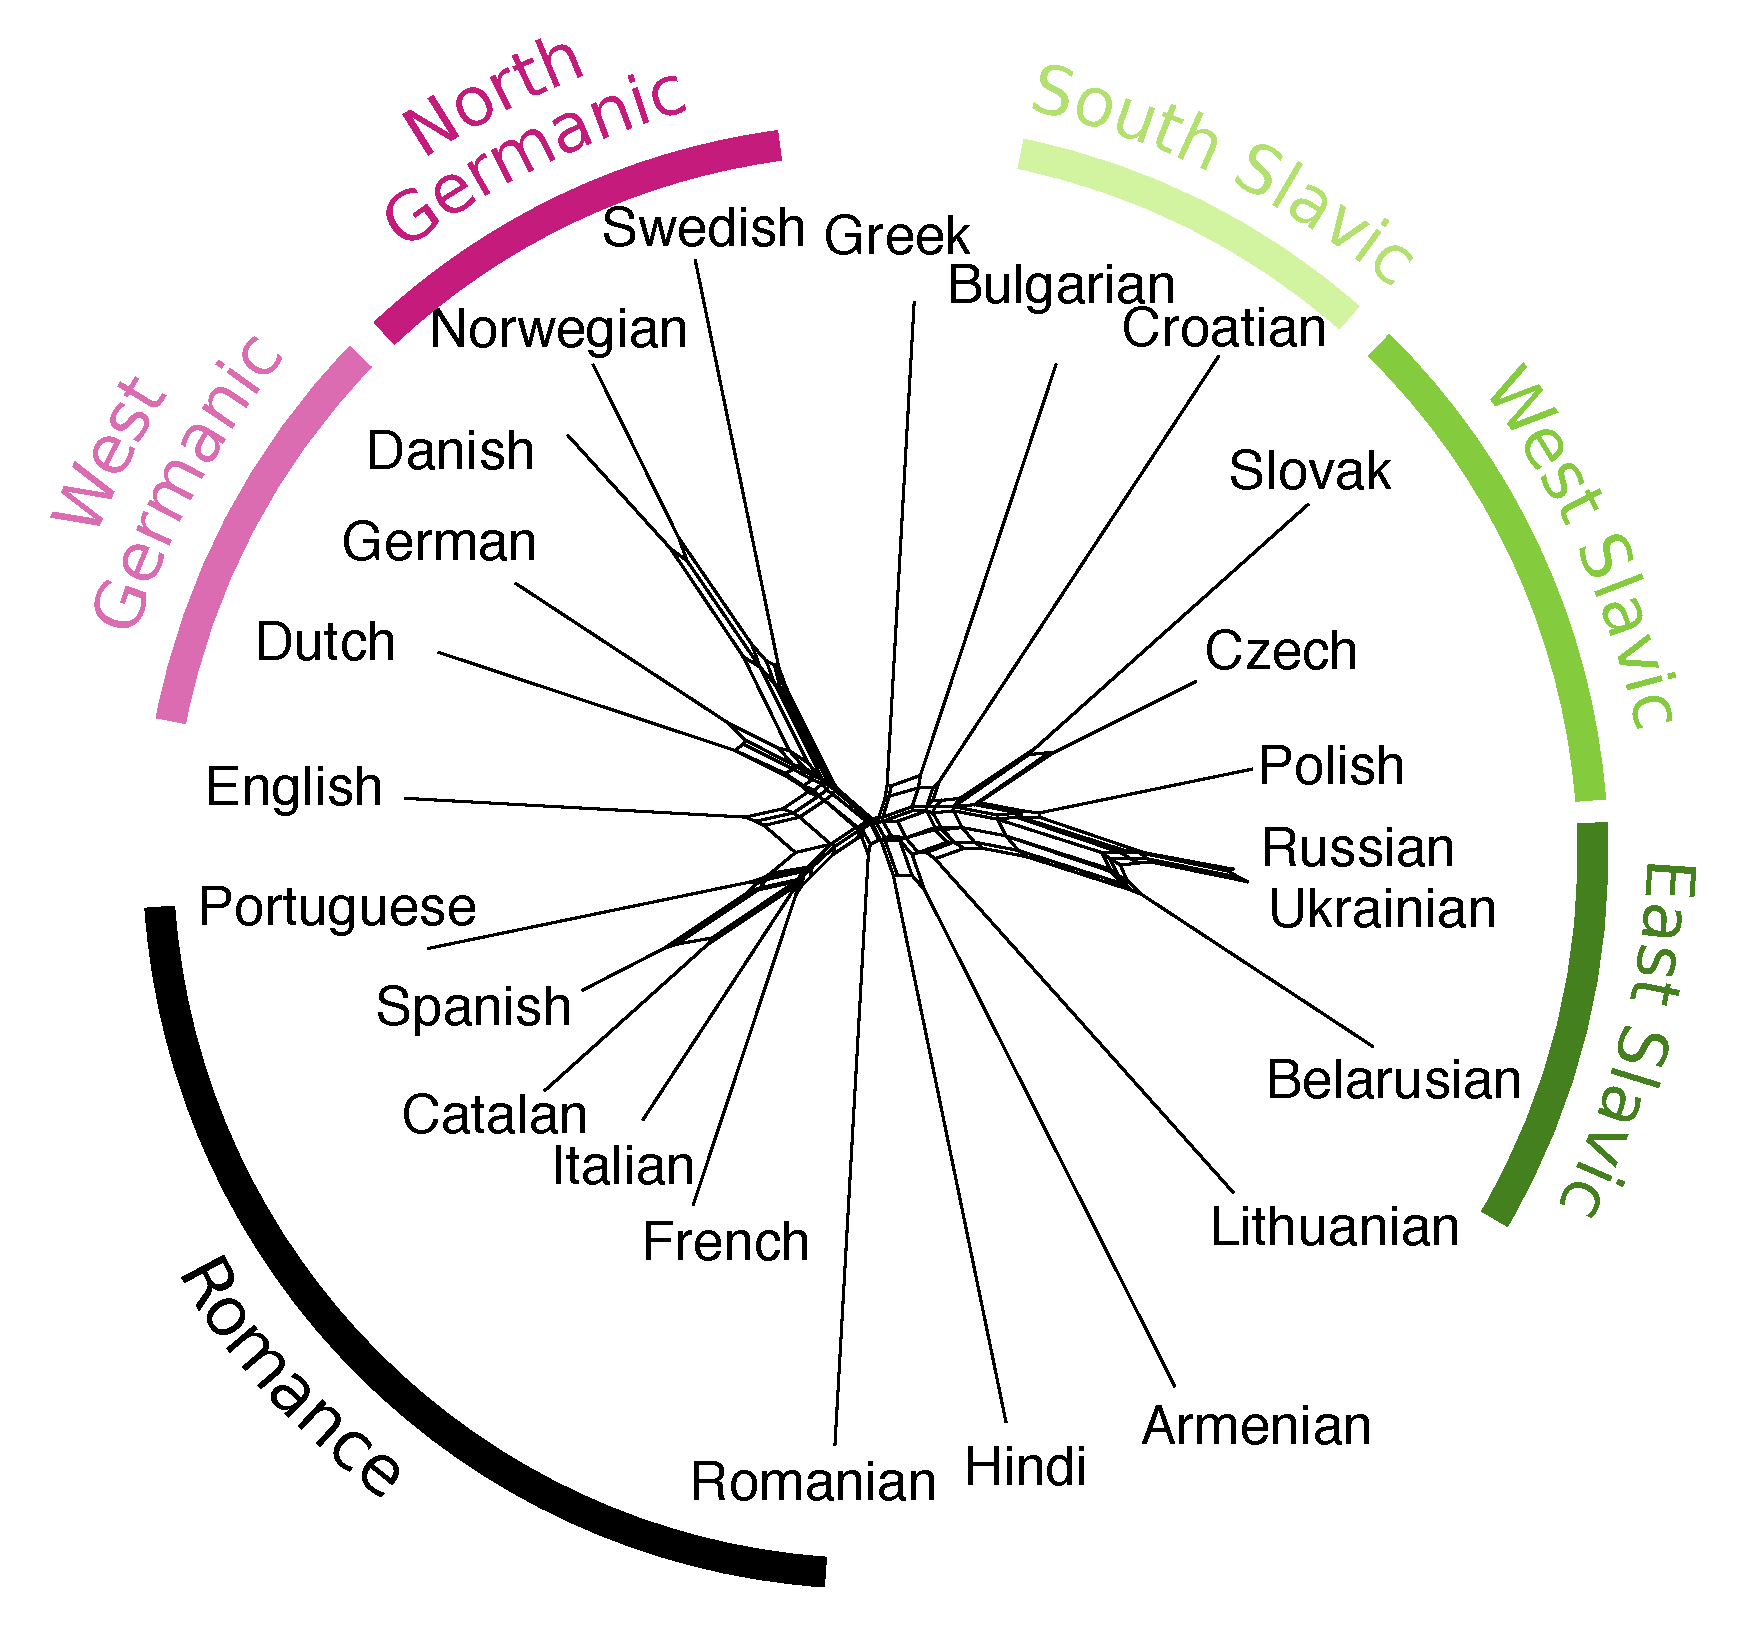
\includegraphics[width=\linewidth]{../results/splitstree/LinguisticDistances_IE_new2.pdf}
\caption{Neighbour Net reflecting semantic distance for Indo-European languages.}
\label{fig:NNIE}
\end{center}
\end{figure}

\clearpage
\newpage
\section{Cross-cultural analysis (Common Crawl data)}

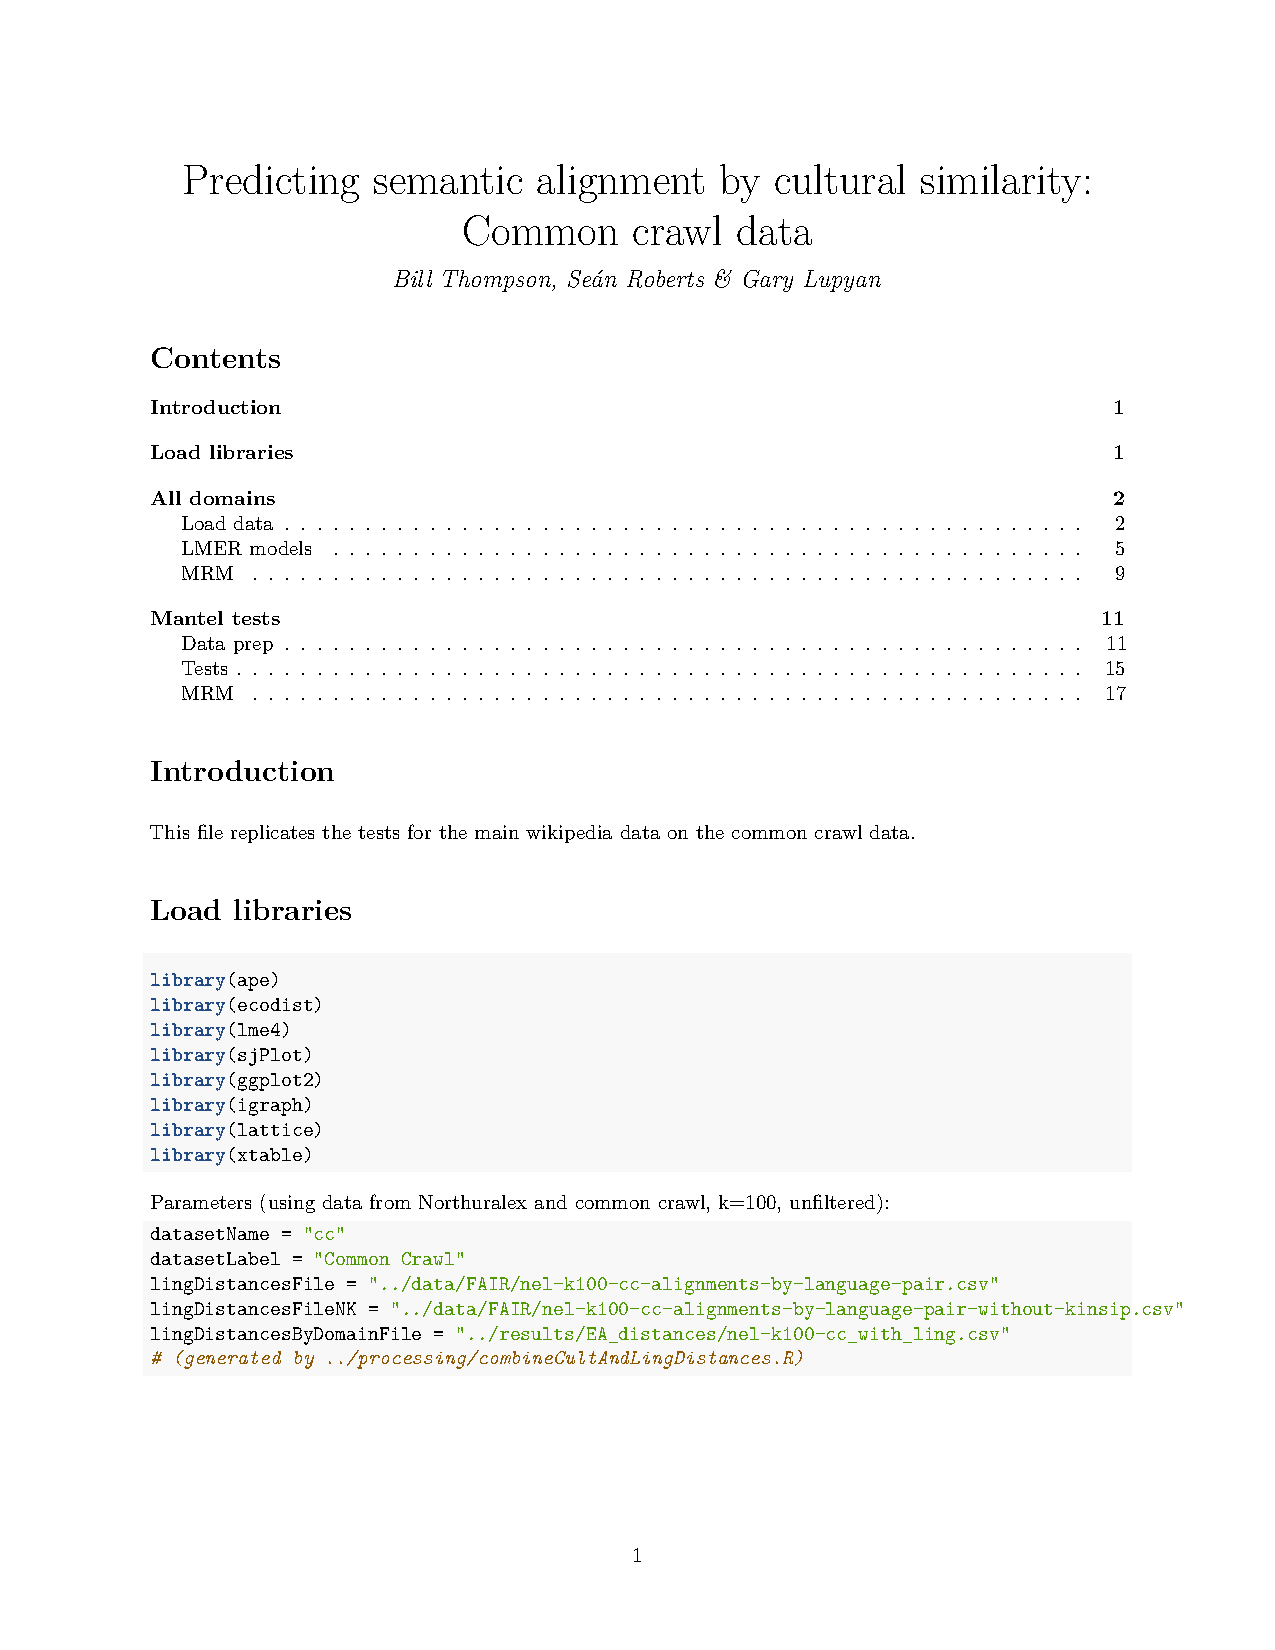
\includepdf[pages=-]{../analysis/AnalyseCorrelation_cc.pdf}

\newpage
\section{Cross-cultural analysis (Subtitles data)}
 
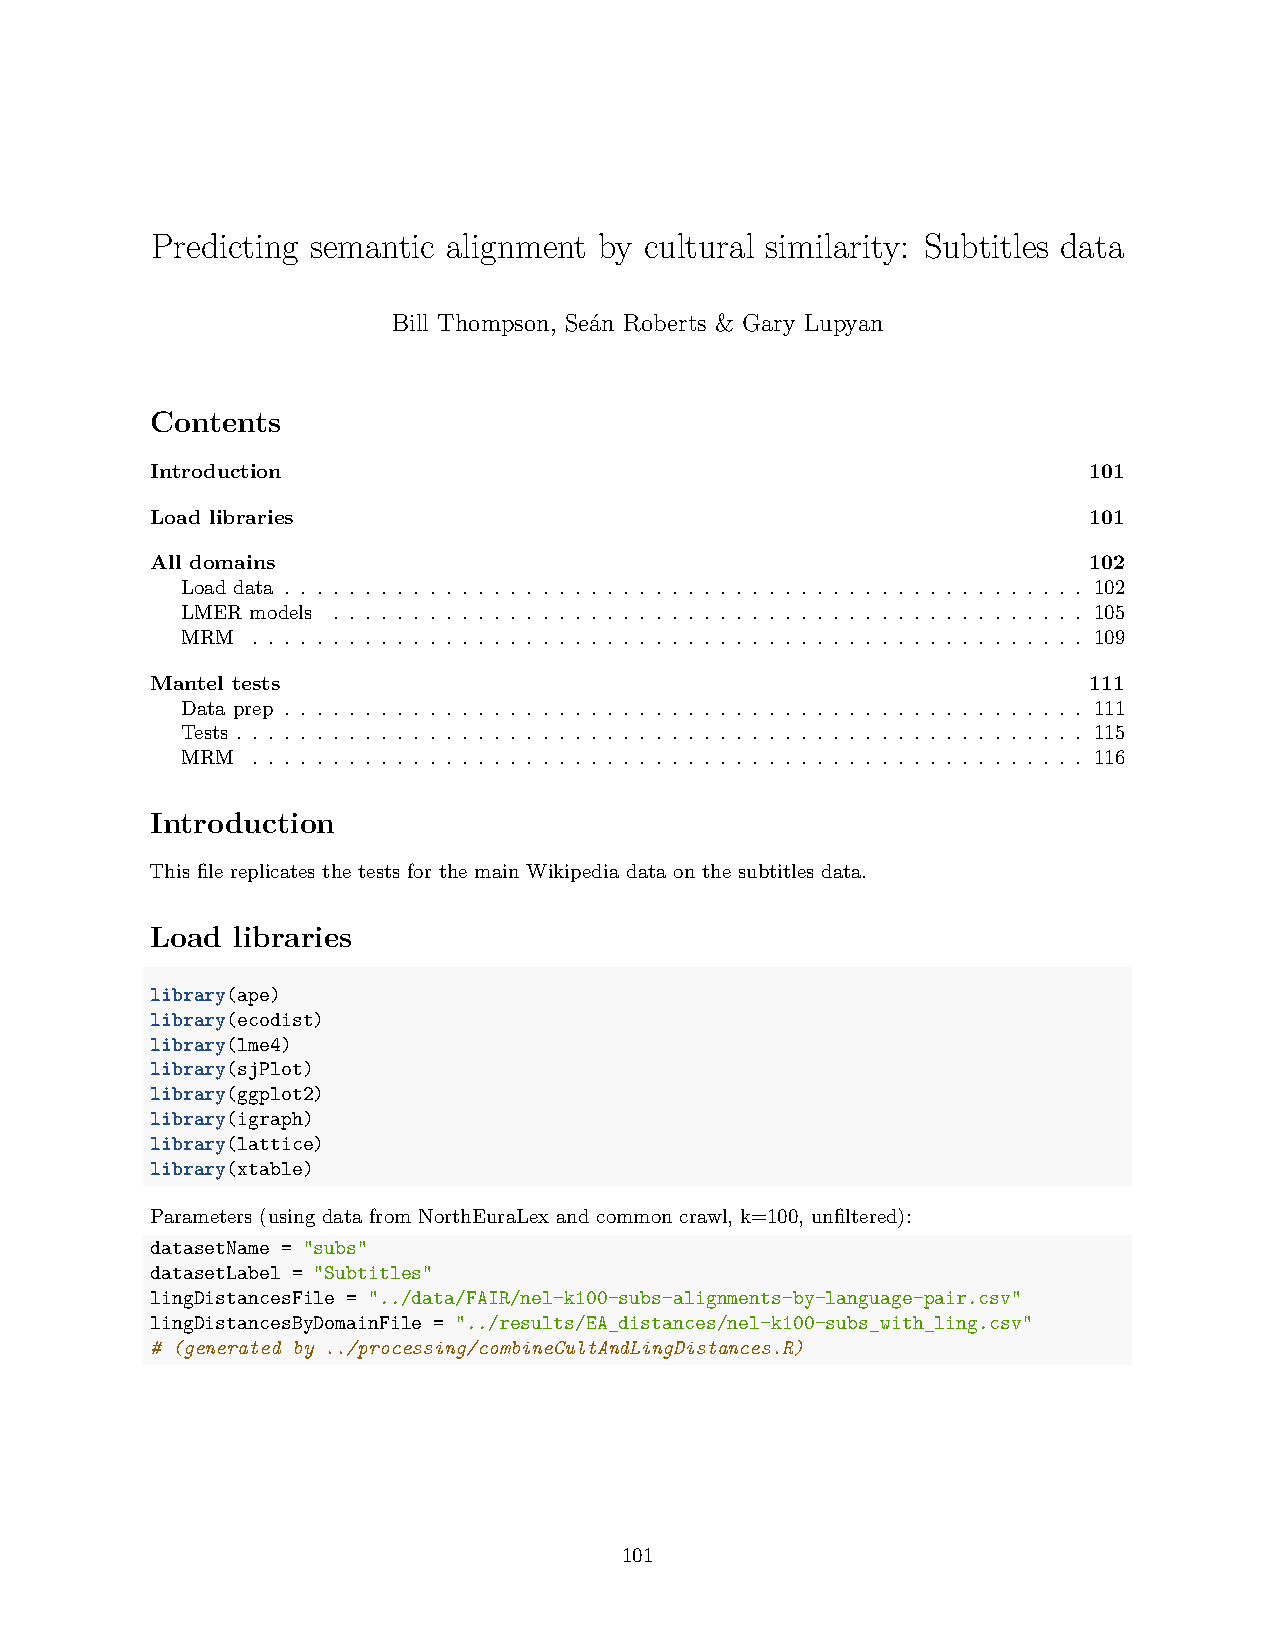
\includepdf[pages=-]{../analysis/AnalyseCorrelation_subs.pdf}

\newpage
\section{Summary of findings}

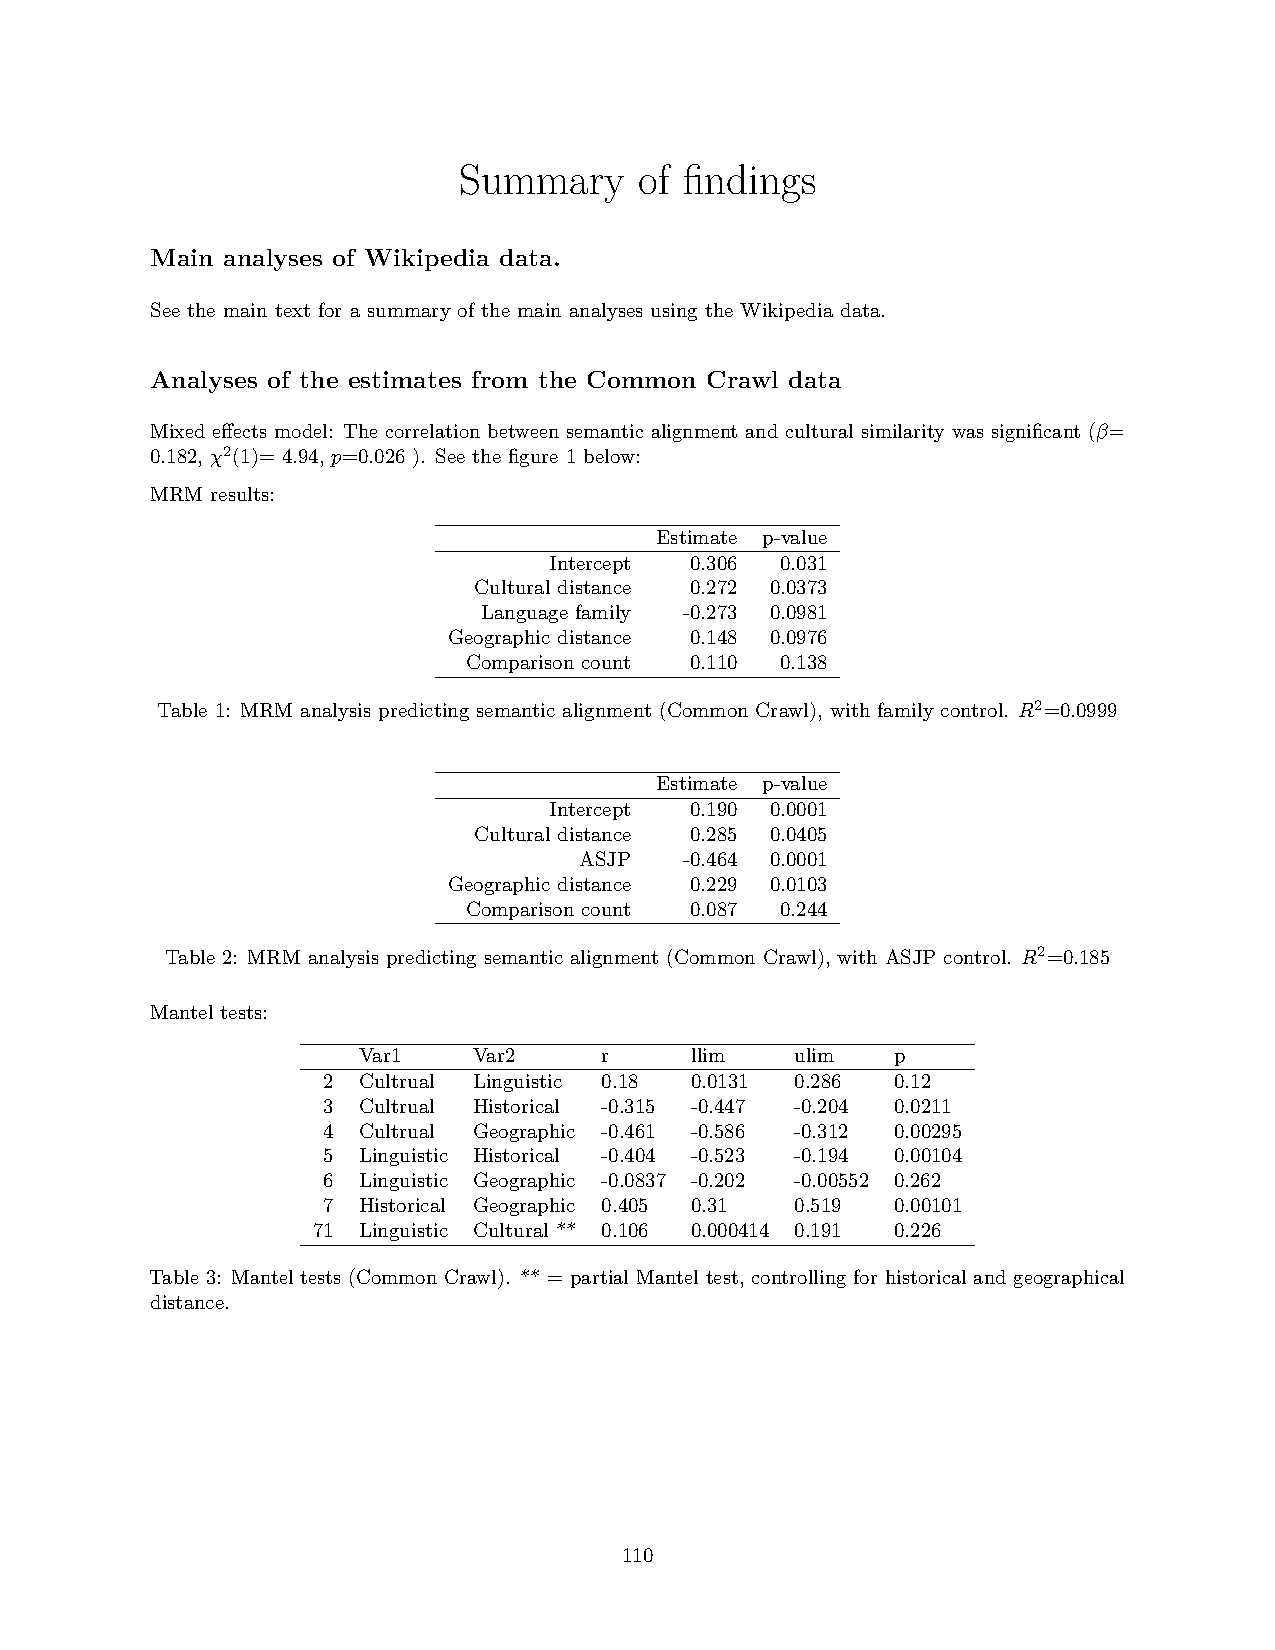
\includepdf[pages=-]{../analysis/SummaryOfFindings.pdf}

\end{document}